\documentclass[tikz,border=5pt]{standalone}
\usepackage{mathpazo}
\usepackage{amsmath}
\usetikzlibrary{arrows.meta}
\begin{document}

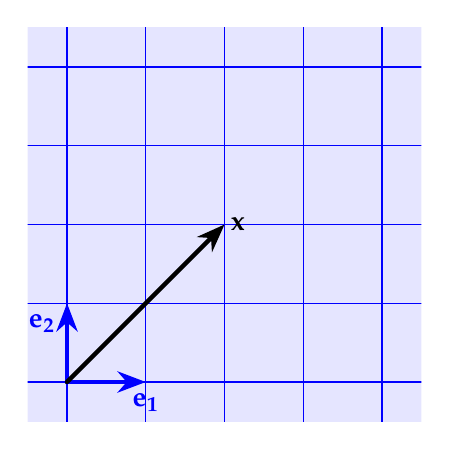
\begin{tikzpicture}[line cap=round]
    \clip (-.5,-.5) rectangle (4.5,4.5);
    \fill[blue!10] (-1,-1) rectangle (5,5);
    \draw[blue] (-1,-1) grid (5,5);
    \draw[blue,ultra thick,-Stealth] (0,0) -- +(1,0) node[below] {$\mathbf{e_1}$};
    \draw[blue,ultra thick,-Stealth] (0,0) -- +(0,1) node[below left] {$\mathbf{e_2}$};
    \draw[black,ultra thick,-Stealth] (0,0) -- +(2,2) node[right=-2pt] {$\mathbf{x}$};
\end{tikzpicture}

% Source - https://tex.stackexchange.com/a/759089
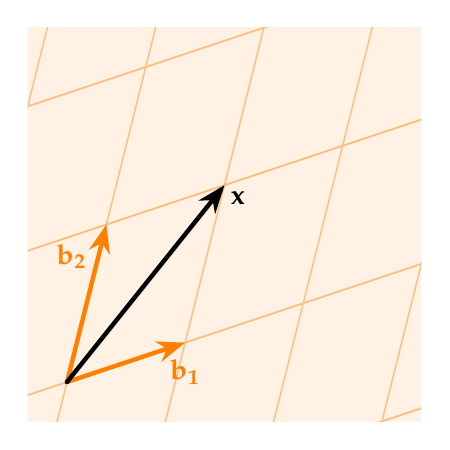
\begin{tikzpicture}[line cap=round]
  \clip (-.5,-.5) rectangle (4.5,4.5);
  \begin{scope}[transform canvas={cm={1.5, 0.5, 0.5, 2, (0,0)}}]
    \fill[orange!10] (-2,-2) rectangle (5,5);
    \draw[orange!50] (-2,-2) grid (5,5);
  \end{scope}
  \begin{scope}[x={(1.5cm,0.5cm)}, y={(0.5cm,2cm)}]
    \draw[orange,ultra thick,-Stealth] (0,0) -- +(1,0) node[below=2pt] {$\mathbf{b_1}$};
    \draw[orange,ultra thick,-Stealth] (0,0) -- +(0,1) node[below left=3pt] {$\mathbf{b_2}$};
    \draw[black,ultra thick,-Stealth] (0,0) -- +(1,1) node[below right=-2pt] {$\mathbf{x}$};
  \end{scope}
\end{tikzpicture}

\end{document}